% mnras_template.tex 
%
% LaTeX template for creating an MNRAS paper
%
% v3.0 released 14 May 2015
% (version numbers match those of mnras.cls)
%
% Copyright (C) Royal Astronomical Society 2015
% Authors:
% Keith T. Smith (Royal Astronomical Society)

% Change log
%
% v3.0 May 2015
%    Renamed to match the new package name
%    Version number matches mnras.cls
%    A few minor tweaks to wording
% v1.0 September 2013
%    Beta testing only - never publicly released
%    First version: a simple (ish) template for creating an MNRAS paper

%%%%%%%%%%%%%%%%%%%%%%%%%%%%%%%%%%%%%%%%%%%%%%%%%%
% Basic setup. Most papers should leave these options alone.
\documentclass[fleqn,usenatbib]{mnras}

% MNRAS is set in Times font. If you don't have this installed (most LaTeX
% installations will be fine) or prefer the old Computer Modern fonts, comment
% out the following line
\usepackage{newtxtext,newtxmath}
% Depending on your LaTeX fonts installation, you might get better results with one of these:
%\usepackage{mathptmx}
%\usepackage{txfonts}

% Use vector fonts, so it zooms properly in on-screen viewing software
% Don't change these lines unless you know what you are doing
\usepackage[T1]{fontenc}

% Allow "Thomas van Noord" and "Simon de Laguarde" and alike to be sorted by "N" and "L" etc. in the bibliography.
% Write the name in the bibliography as "\VAN{Noord}{Van}{van} Noord, Thomas"
\DeclareRobustCommand{\VAN}[3]{#2}
\let\VANthebibliography\thebibliography
\def\thebibliography{\DeclareRobustCommand{\VAN}[3]{##3}\VANthebibliography}


%%%%% AUTHORS - PLACE YOUR OWN PACKAGES HERE %%%%%

% Only include extra packages if you really need them. Common packages are:
\usepackage{graphicx, caption, subcaption}	% Including figure files
\usepackage{amsmath}	% Advanced maths commands
\usepackage{amssymb}	% Extra maths symbols

%%%%%%%%%%%%%%%%%%%%%%%%%%%%%%%%%%%%%%%%%%%%%%%%%%

%%%%% AUTHORS - PLACE YOUR OWN COMMANDS HERE %%%%%

% Please keep new commands to a minimum, and use \newcommand not \def to avoid
% overwriting existing commands. Example:
%\newcommand{\pcm}{\,cm$^{-2}$}	% per cm-squared

%%%%%%%%%%%%%%%%%%%%%%%%%%%%%%%%%%%%%%%%%%%%%%%%%%

%%%%%%%%%%%%%%%%%%% TITLE PAGE %%%%%%%%%%%%%%%%%%%

% Title of the paper, and the short title which is used in the headers.
% Keep the title short and informative.
\title[Al-26 from Interacting Binaries]{Aluminium-26 Ejection from Massive Interacting Binary Stars}


% The list of authors, and the short list which is used in the headers.
% If you need two or more lines of authors, add an extra line using \newauthor
\author[L. R. Humphrey]{
Luke R. Humphrey$^{1}$%\thanks{}
%, A. N. Other$^{2}$
%, Third Author$^{2,3}$
% and Fourth Author$^{3}$
\\
% List of institutions
$^{1}$University of Hull, Cottingham Rd, Hull HU6 7RX, UK\\
}

% These dates will be filled out by the publisher
\date{Accepted XXX. Received YYY; in original form ZZZ}

% Enter the current year, for the copyright statements etc.
\pubyear{2020}

% Don't change these lines
\begin{document}
\label{firstpage}
\pagerange{\pageref{firstpage}--\pageref{lastpage}}
\maketitle

% Abstract of the paper
\begin{abstract}
% Background.
In a close binary system, mass can be stripped from the surface of one star and accreted onto its companion.
This can alter the stellar wind chemical yields of both stars due to the resulting change in surface composition and direct ejection of material during the mass transfer.
% Al-26
Aluminium-26 ($^{26}$Al), an isotope produced in core hydrogen-burning but destroyed in core helium-burning, is not usually ejected in large quantities by massive single stars before the supernova.
In binary systems, however, mass transfer before the end of helium-burning can eject deep layers of $^{26}$Al.
% What we did.
In this study, we modelled the evolution of non-rotating massive binaries to investigate $^{26}$Al yields while varying period P and mass transfer efficiency $\beta$.
% What we found.
The initial period of the system was found to affect how soon, if at all, mass transfer occurred.
$^{26}$Al yields for binary systems with initial masses 20 \& 18 M$_{\sun}$ were found to increase due to mass transfer between hydrogen and helium-burning in the mass-losing star. Yields were not significantly affected if mass transfer occurred during helium-burning.
In addition, yields were not affected in systems with initial masses 50 \& 45 M$_{\sun}$ since stars of this mass eject their envelope as they evolve into Wolf-Rayet stars.
Varying $\beta$ decreased yields for the mass-losing star as a higher fraction was accreted onto the companion.
With more accreted material, companion stars were found to have increased yields which, if allowed to complete their evolution, outweighed the reduction in yields for the mass-losing star.
\end{abstract}

% Select between one and six entries from the list of approved keywords.
% Don't make up new ones.
\begin{keywords}
method: numerical -- stars: evolution, mass-loss, winds -- binaries: general
\end{keywords}

%%%%%%%%%%%%%%%%%%%%%%%%%%%%%%%%%%%%%%%%%%%%%%%%%%

%%%%%%%%%%%%%%%%% BODY OF PAPER %%%%%%%%%%%%%%%%%%

\section{Introduction} % Approx word count = 1000 words (total = 1250)

% Al26 Intro & Observations
Aluminium-26 ($^{26}$Al) is a relatively long-lived, radioactive isotope with a half life of $\lambda = 0.72$ Myrs \citep{Iliadis2015}.
It is observed in the Galaxy via $\gamma$-ray spectroscopy of its 1.81 MeV decay to $^{26}$Mg \citep{2004ESASP.552...27D}.
An excess of $^{26}$Mg has been found in meteorite samples \citep{1978ApJ...224L.139A} and pre-solar grains \citep{2011ApJS..193...16I}, indicating that more $^{26}$Al was present in the early solar system than the current galactic average \citep[see][]{2019ApJ...884...38B}.
\cite{2011ApJS..193...16I} note that ``the observation of Galactic $\gamma$-rays from $^{26}$Al is important since it provides unambiguous direct evidence for ... nucleosynthesis in stars'' even if ``the origin of $^{26}$Al remains controversial''.

\subsection{Aluminium-26 Production in Stars}

% Stellar evolution
% Stars are created in galaxies from material in the interstellar medium (ISM). Nuclear reactions in stars alters the composition of this material as they evolve. Ultimately, when a star dies, this material is returned to the ISM and goes on to create new generations of stars. The resulting evolution of chemical composition in galaxies is called galactic chemical evolution (GCE).
% Stellar nucleosynthesis is responsible for creating almost all elements beyond hydrogen and helium\footnote{Excepting man-made elements and elements formed in the ISM by cosmic ray spallation.} and also keeps stars stable during their lifetimes: energy released from fusion generates an outward thermal pressure that comes into hydrostatic equilibrium with the inwards pressure of the star's own weight.

Stars spend most of their lives on the main sequence, generating energy from hydrostatic fusion of $^1$H into $^4$He in the core.
Hydrogen-burning reactions range from the simple proton-proton chains dominant in low mass stars, to cycles of proton-capture and $\alpha$-decay reactions that use heavier elements as catalysts such as the CNO cycle dominant in high mass stars \citep{Iliadis2015}.

After exhausting hydrogen in the core, the stellar envelope cools and expands as the core contracts and heats up. Meanwhile, hydrogen-burning continues in a shell layer around the core.
With sufficient mass, stellar cores can reach temperatures high enough to fuse heavier elements, the first of which is helium.
Depending on their initial mass, stars can burn through carbon, neon, oxygen, and ultimately silicon.
Massive stars end their lives in core collapse supernovae (CCSN), leaving behind a neutron star or a black hole \citep{Carroll2007}.

\begin{figure}
    \centering
    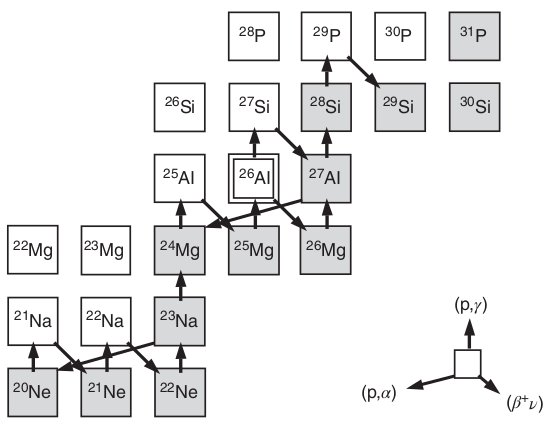
\includegraphics[width=\columnwidth]{figures/intro/AlMg.png}
    \captionsetup{width=0.9\columnwidth}
    \caption{The hydrogen-burning neon-sodium (Ne-Na) \& aluminium-magnesium (Al-Mg) cycles represented on the chart of nuclides.
    The orientation of each arrow represents a particular reaction: proton capture ($\mathrm{p,\gamma}$), $\mathrm{\beta^+}$ decay ($\mathrm{\beta^+\nu}$), and helium emission ($\mathrm{p,\alpha}$).
    Diagram from \cite{Iliadis2015}.}
    \label{fig:reactions}
\end{figure}

% Al26 Production and Destruction
In massive stars, $^{26}$Al is created in both core and shell hydrogen burning via the Al-Mg cycle (see figure \ref{fig:reactions}): a catalytic series of reactions similar to the CNO cycle.
In the absence of production channels, $^{26}$Al decays to $^{26}$Mg during helium-burning and is also destroyed via neutron capture reactions \citep{2019ApJ...884...38B}.
It is later produced in carbon and neon-burning convective shells \citep{1978ApJ...224L.139A} and ejected in the supernova, which synthesises additional $^{26}$Al via explosive neon-burning \citep{2006ApJ...647..483L}.
These latter sources are by far the largest contributor to stellar $^{26}$Al yields\footnote{A star's isotope `yield' is defined as the mass of that isotope ejected from the star over its lifetime. Pre-supernova yields can be calculated by integrating the surface abundance of the isotope multiplied by the surface mass-loss rate with respect to time.}.

% Al26 isomer
$^{26}$Al can be formed either in its ground state $^{26}$Al$^g$ or an isomeric\footnotemark state $^{26}$Al$^m$.
While most isotopes come into thermal equilibrium with their excited states, $^{26}$Al represents a rare exception and does not reach equilibrium below T = 0.4 GK \citep{Iliadis2015}. Thus each state is considered individually during the hydrogen-burning stage. 
\footnotetext{An isomeric state is a relatively long lived excited state with a half life on the order of seconds to days.}
In this paper, $^{26}$Al is used to refer exclusively to $^{26}$Al$^g$; we are not concerned with $^{26}$Al$^m$ since it decays too quickly for it to contribute meaningfully to $^{26}$Al yields.

% Ejecting Al26 with winds
Stellar winds eject material from the surface into the interstellar medium (ISM).
Main sequence winds are not usually strong enough to extract much $^{26}$Al, but helium-burning winds can eject $^{26}$Al produced in shell hydrogen burning layers and in some cases much of the $^{26}$Al left over from the main sequence.
Stars with initial mass greater than ~20 M$_{\sun}$ regularly eject their entire envelopes and hydrogen-burning shells, becoming a Wolf-Rayet (WR) star \citep{Carroll2007}.

% Ejecting Al26 with RLOF
Another way in which stars eject material is through mass transfer with a binary companion.
Since $^{26}$Al is created during hydrogen-burning and destroyed during helium-burning, mass transfer must occur between zero-age main sequence (ZAMS) and the end of helium-burning in order to contribute significantly to $^{26}$Al yield.

\subsection{Aluminium-26 from Binary Stars}

\begin{figure}
    \centering
    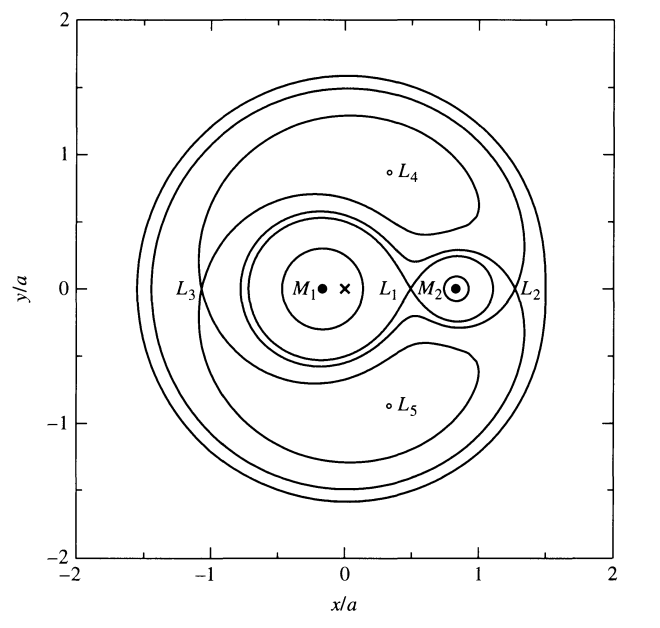
\includegraphics[width=\columnwidth]{figures/intro/RL.png}
    \captionsetup{width=0.9\columnwidth}
    \caption{Equipotential lines around a binary system consisting of stars M$_1$ and M$_2$. The $\times$ marks the centre of mass, while L$_1$ is the zero-potential inner-Lagrangian point between both stars. Note that the equipotential lines passing through this point define the Roche lobes of each star.
    Diagram from \cite{Carroll2007}}
    \label{fig:RocheLobes}
\end{figure}

A binary system consists of two stars orbiting their centre of mass.
Their mean separation can vary greatly, with distant binaries experiencing little to no interaction.
Tidal effects in close binaries bring the stars closer together \citep[see][]{Iliadis2015}, increasing the likelihood of mass transfer, or even common envelope evolution\footnote{Common envelope evolution occurs when binary stars are close enough to physically overlap.}.
There is still uncertainty as to what proportion of stars exist as part of an interacting binary system.
However, \cite{2012Sci...337..444S} found that binary interactions are the norm for massive stars, with over 70\% experiencing mass transfer at some point in their evolution.

There are two processes responsible for binary mass transfer: stellar winds\footnote{The effects of wind mass transfer are minimal compared to RLOF, as only a very small fraction of mass lost by stellar winds is accreted onto the companion.} and Roche lobe overflow (RLOF).
The latter occurs when a star in a binary system, usually the primary\footnote{Since the first major expansion in stellar radius occurs after the main-sequence and more massive stars evolve faster than lower mass stars, it is more likely for the more massive primary to enter RLOF before the secondary.}, expands beyond the central zero-potential point $L_1$\footnote{$L_1$ is called the inner Lagrangian point and is situated at a point between the stars where the gravitational potential of both stars cancels to zero. There are also four outer Lagrangian points ($L_2$ through $L_5$) in a binary system.}.
Figure \ref{fig:RocheLobes} depicts the gravitational equipotential surfaces around binary stars; such surfaces are spherical around a single star, but in binaries they are deformed towards $L_1$ to form teardrop-shaped Roche lobes which together define a three-dimensional figure-8 \citep{Iliadis2015}.

When a star fills its Roche lobe, material is stripped from the surface, through $L_1$, and into the Roche lobe of its companion.
From here, the lost material is either accreted onto the companion or ejected into the ISM.
The fraction of the mass lost that is accreted onto the companion is called the mass transfer efficiency $\beta$\footnotemark, ranging from $\beta = 1$ (fully conservative) to $\beta = 0$ (fully non-conservative).
\footnotetext{In this paper, $\beta$ is used to denote the fraction of the mass lost from the mass-losing star that is accreted onto the partner star during RLOF. Please note that other documents, including \cite{2019ApJ...884...38B}, use $1 - \beta$ to mean the same thing.}
Mass transfer through RLOF is further classified based on the evolutionary stage of the mass-losing star: case A for the main-sequence, C for helium-burning, and B for the Hertzsprung gap between these stages.

\subsection{Aims of This Study}

This study investigates the effects of mass transfer on the $^{26}$Al production of massive binary stars compared to their single star counterparts.
$^{26}$Al production in massive binaries was recently studied by \cite{2019ApJ...884...38B} who found that the effects of binary interaction can differ dramatically depending on various parameters.
%
Here, we investigate the effects of the initial masses, orbital period, and mass transfer efficiency.
While the focus is on $^{26}$Al, the processes observed in these simulations may be of use for binary studies for any isotope.
We also aim to demonstrate the potential for binary phenomena to impact stellar nucleosynthesis and to stress the role of binaries in galactic chemical evolution. % ~ 880/ 750 (+130)
\section{Method} % Approx word count = 500 words

% STARS Overview
Non-rotating binary star systems were simulated using the stellar evolution and nucleosynthesis code STARS.
STARS is a one-dimensional code capable of evolving stars up to core-collapse.
The code simulates the evolution of both composition and structure of stellar models simultaneously to converge the model at each timestep.

STARS was originally written by \cite{1971MNRAS.151..351E}, and has been updated many times since then \citep[e.g.][]{1995MNRAS.274..964P}.
The version used here is from \cite{2009MNRAS.396.1699S}, who added the functionality to evolve binary systems.
% This version follows the chemical evolution of 46 species (including both isomeric $^{26}$Al$^m$ \& ground state $^{26}$Al$^g$).

STARS uses a simple diffusion model described in \cite{1972MNRAS.156..361E} to simulate mixing.
Overshooting of convective region boundaries is used to compensate for the additional mixing found in observations (see \cite{1991A&AS...89..451M} for why this is necessary). Note that the additional observed mixing is likely to result from multiple effects, not just mixing beyond the theoretical boundaries \citep{2015A&A...575A.117S}.

\subsection{Simulation Parameters} \label{Method2}

% Simulation parameters
The simulations were run using ZAMS stellar models; initial compositions were set to solar values.
The mixing length (used for convective overshooting) was set to 2.0 in all simulations, after the Solar model calibrations used by \cite{2015A&A...575A.117S}.
Preliminary testing on spacial and temporal resolution was done to maximise the speed of each run without sacrificing accuracy: all simulations in this study used 199 mesh points and variable timesteps.
We use the updated Wolf-Rayet mass loss rates described in \cite{Eldridge2006}; this system uses rates from \cite{MassLossRates1} for OB stars, \cite{MassLossRates2} for pre-WR stars, and \cite{MassLossRates3} for WR stars.

Mass transfer efficiency $\beta = 0.5$ is used, except where stated otherwise. Mass lost from the primary (through RLOF or winds) is accreted onto the secondary at this fraction.
As mass is transferred, so is the angular momentum associated with that mass. This tends to increase the rotational velocity of the secondary star during mass transfer. As the angular frequency approaches a critical value, the mass loss rate increases while $\beta$ drops off rapidly. 
The code's treatment of this phenomenon is discussed in detail in \cite{2009MNRAS.396.1699S}.

% Stellar Model Parameters
Single and binary star simulations were run for systems with initial primary masses 20 M$_{\sun}$ \& 50 M$_{\sun}$, with mass ratio $q$ = $\frac{M_2}{M_1}$ = 0.9 (i.e. initial secondary star masses of 18 M$_{\sun}$ \& 45 M$_{\sun}$). These values follow \cite{2019ApJ...884...38B}, to allow a direct comparison of results.
Except where stated, the initial orbital periods used were P = 100 days for binaries and P = 10$^{77}$ for single stars\footnote{Note that when evolving two models at once, the code always treats both stars as existing in a binary system. Single star evolution is simulated by using an arbitrarily high period (and thus separation) which prevents interaction between the stars.}.       % ~ 350/ 250 (+100)
\section{Results} % Approx word count = 1000 words (total = 2750)

\begin{figure*}
    \centering
    \begin{subfigure}{\columnwidth}
        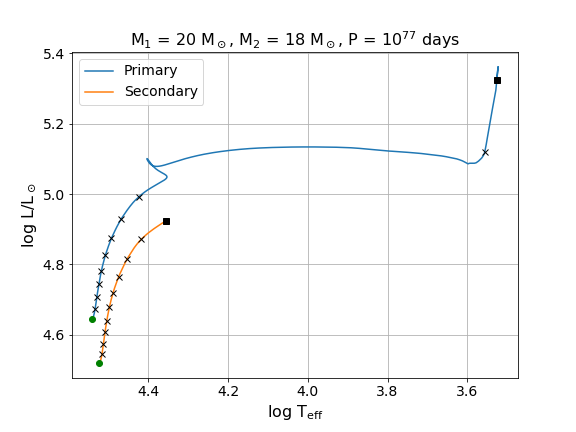
\includegraphics[width=\textwidth]{figures/results1/fig_HR_M20_Sin.png}
        \captionsetup{width=.9\columnwidth}
        \caption{HR diagram showing the evolution tracks for the M$_1$ = 20 M$_{\sun}$ system as non-interacting single stars.
        Note both tracks terminate simultaneously when the primary completes core helium burning.}
        \label{subfig:20Msol_HR_Sin}
    \end{subfigure}
    \hfill
    \begin{subfigure}{\columnwidth}
        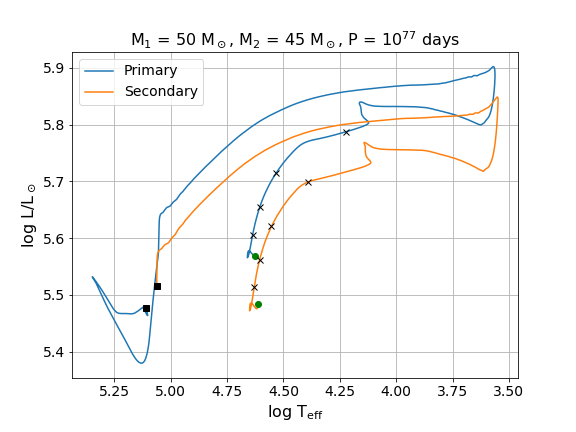
\includegraphics[width=\textwidth]{figures/results1/fig_HR_M50_Sin.png}
        \captionsetup{width=.9\columnwidth}
        \caption{As figure \ref{subfig:20Msol_HR_Sin} for the M$_1$ = 50 M$_{\sun}$ system. \newline \newline}
        \label{subfig:50Msol_HR_Sin}
    \end{subfigure}
    
    \begin{subfigure}{\columnwidth}
        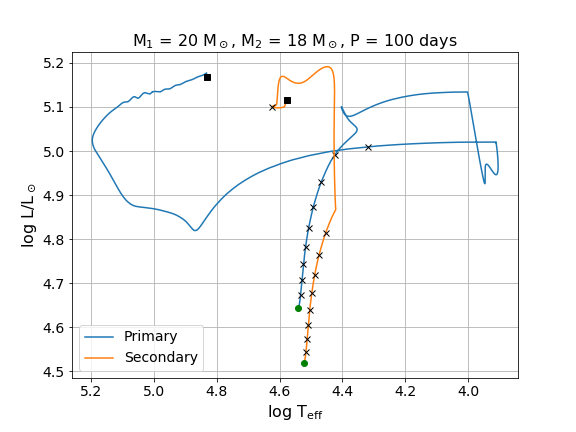
\includegraphics[width=\columnwidth]{figures/results1/fig_HR_M20_P100.png}
        \captionsetup{width=.9\columnwidth}
        \caption{HR diagram showing the evolution tracks for the M$_1$ = 20 M$_{\sun}$ interacting binary system at initial period P = 100 days.}
        \label{subfig:20Msol_HR_Bin}
    \end{subfigure}
    \hfill
    \begin{subfigure}{\columnwidth}
        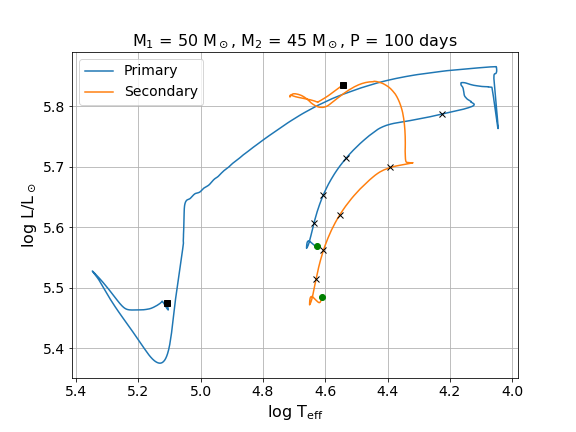
\includegraphics[width=\columnwidth]{figures/results1/fig_HR_M50_P100.png}
        \captionsetup{width=.9\columnwidth}
        \caption{As figure \ref{subfig:20Msol_HR_Bin} for the M$_1$ = 50 M$_{\sun}$ system. \newline}
        \label{subfig:50Msol_HR_Bin}
    \end{subfigure}
    
    \begin{subfigure}{\columnwidth}
        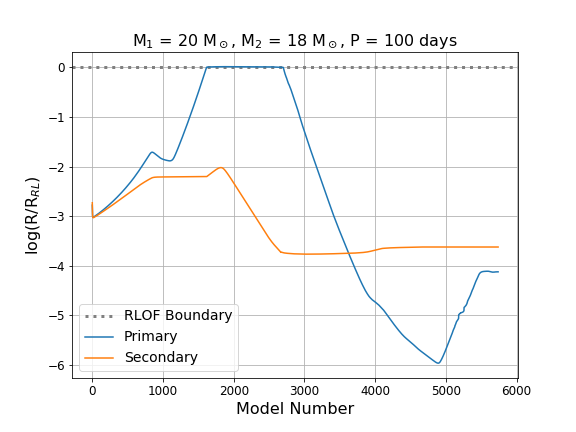
\includegraphics[width=\columnwidth]{figures/results1/fig_RLOF_M20_P100.png}
        \captionsetup{width=.9\columnwidth}
        \caption{Stellar radius as a fraction of Roche lobe radius for the M$_1$ = 20 M$_{\sun}$ system. Roche lobe overflow occurs while $\log$(R/R\textsubscript{RL}) = 0.}
        \label{subfig:20Msol_RLOF}
    \end{subfigure}
    \hfill
    \begin{subfigure}{\columnwidth}
        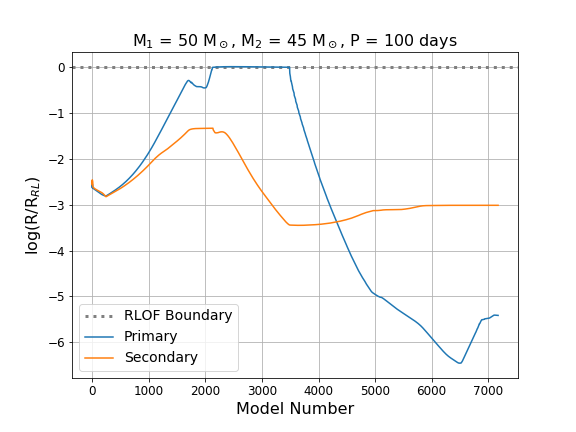
\includegraphics[width=\columnwidth]{figures/results1/fig_RLOF_M50_P100.png}
        \captionsetup{width=.9\columnwidth}
        \caption{As figure \ref{subfig:20Msol_RLOF} for the M$_1$ = 50 M$_{\sun}$ system. \newline}
        \label{subfig:50Msol_RLOF}
    \end{subfigure}
\caption{Diagrams comparing the evolution of M$_1$ = 20 M$_{\sun}$ (left) and M$_1$ = 50 M$_{\sun}$ (right) binary systems with their single star counterparts. The HR evolution tracks begin at the green circle as zero-age main sequence stars, each $\times$ marks 10$^6$ years of evolution. Note that the stellar radius plots are shown in terms of the simulation model number (i.e. non-linear timesteps) to give a qualitative impression of the RLOF process (which happens on a very short timescale relative to the age of the star).}
\label{fig:SinglevsBinary}
\end{figure*}

\begin{figure*}
    \centering
    \begin{subfigure}{\columnwidth}
        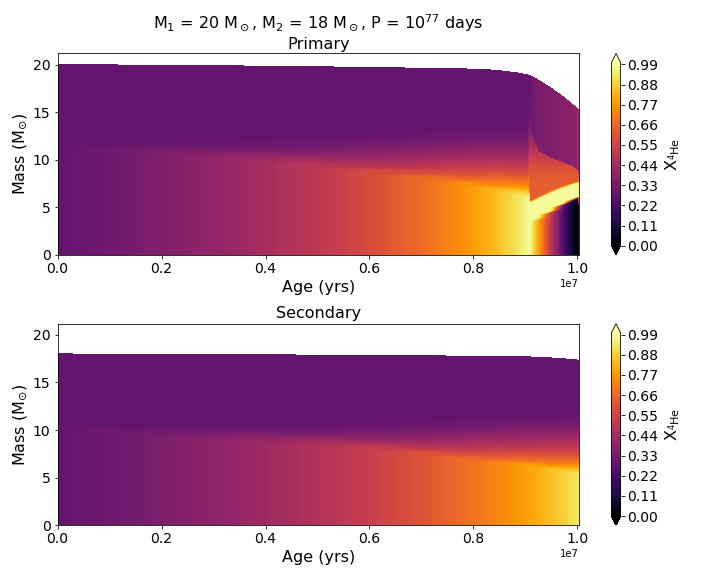
\includegraphics[width=\textwidth]{figures/results1/fig_He4_Age_M20_Sin.png}
        \captionsetup{width=.9\columnwidth}
        \caption{He-4 composition for the single star simulation.}
        \label{subfig:20Msol_He4_Sin}
    \end{subfigure}
    \begin{subfigure}{\columnwidth}
        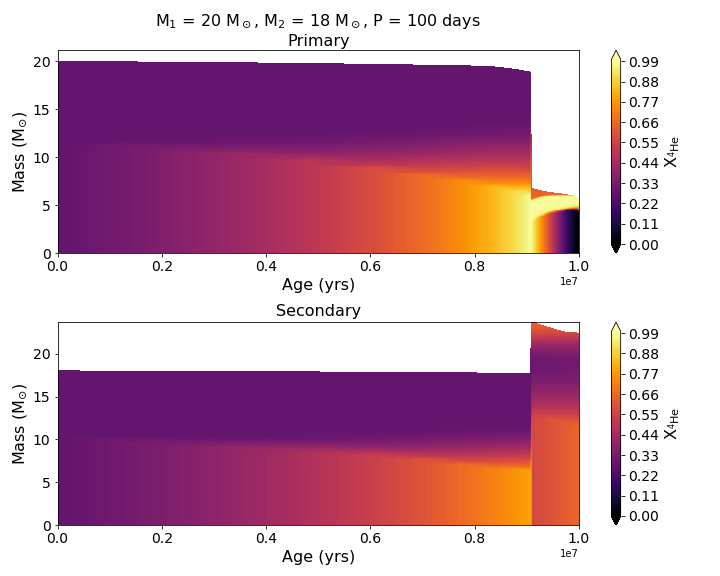
\includegraphics[width=\textwidth]{figures/results1/fig_He4_Age_M20_P100.png}
        \captionsetup{width=.9\columnwidth}
        \caption{He-4 composition for the P = 100 days binary simulation.}
        \label{subfig:20Msol_He4_Bin}
    \end{subfigure}
    \begin{subfigure}{\columnwidth}
        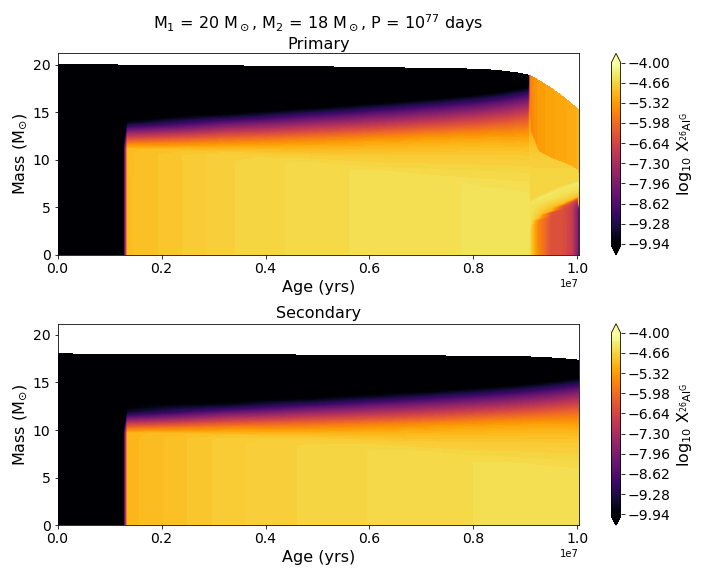
\includegraphics[width=\textwidth]{figures/results1/fig_Al26_Age_M20_Sin.png}
        \captionsetup{width=.9\columnwidth}
        \caption{$^{26}$Al composition for the single star simulation.}
        \label{subfig:20Msol_Al26_Sin}
    \end{subfigure}
    \begin{subfigure}{\columnwidth}
        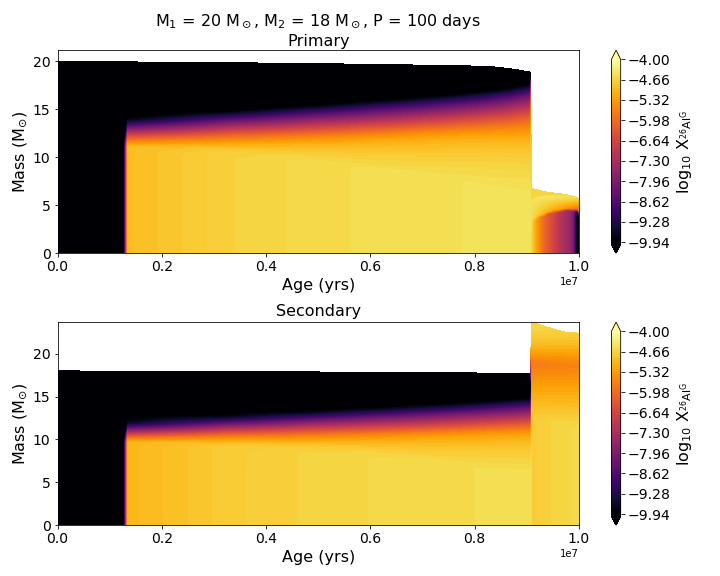
\includegraphics[width=\textwidth]{figures/results1/fig_Al26_Age_M20_P100.png}
        \captionsetup{width=.9\columnwidth}
        \caption{$^{26}$Al composition for the P = 100 days binary simulation.}
        \label{subfig:20Msol_Al26_Bin}
    \end{subfigure}
\caption{Figures showing the chemical evolution of the M$_1$ = 20 M$_{\sun}$ system as single stars (left) and binary stars with initial period 100 days (right).
The y-axis shows the mass of the star, while the colour gives the composition for material in the star at that mass coordinate(i.e. at the radius for which a sphere of that radius centred on the stellar core would contain a given mass).
Note that He-4 and $^{26}$Al are both created in hydrogen-burning stages and destroyed in helium-burning stages.
}
\label{fig:20Msol_Composition}
\end{figure*}

\begin{figure*}
    \begin{subfigure}{\columnwidth}
        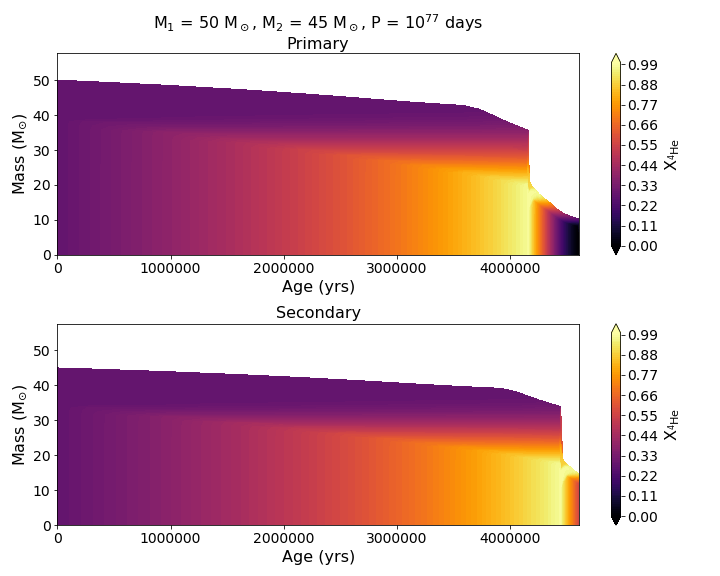
\includegraphics[width=\textwidth]{figures/results1/fig_He4_Age_M50_Sin.png}
        \captionsetup{width=.9\columnwidth}
        \caption{He-4 composition for the single star simulation.}
        \label{subfig:50Msol_He4_Sin}
    \end{subfigure}
    \begin{subfigure}{\columnwidth}
        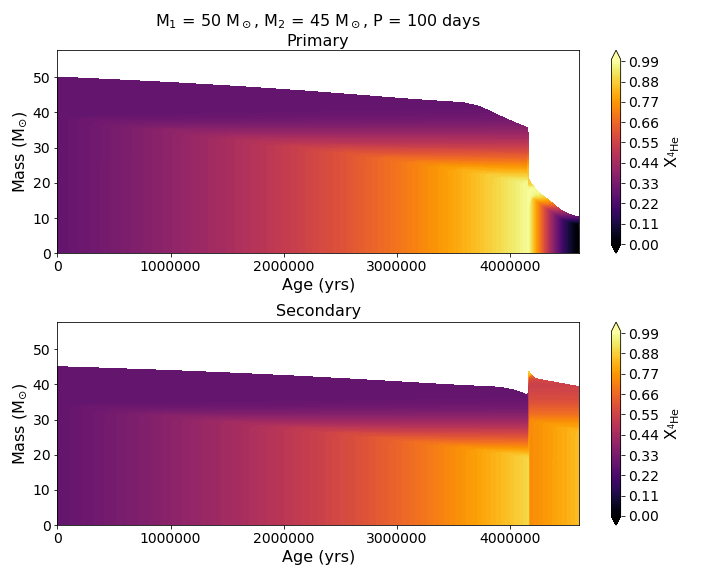
\includegraphics[width=\textwidth]{figures/results1/fig_He4_Age_M50_P100.png}
        \captionsetup{width=.9\columnwidth}
        \caption{He-4 composition for the P = 100 days binary simulation.}
        \label{subfig:50Msol_He4_Bin}
    \end{subfigure}
    \begin{subfigure}{\columnwidth}
        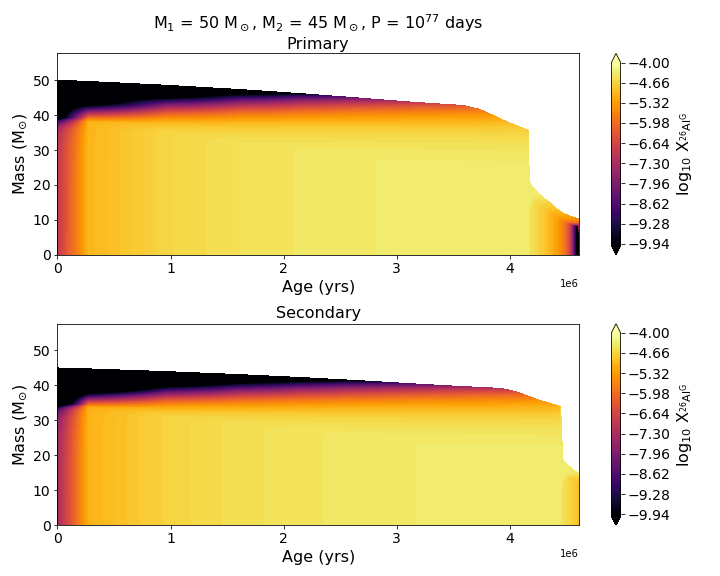
\includegraphics[width=\textwidth]{figures/results1/fig_Al26_Age_M50_Sin.png}
        \captionsetup{width=.9\columnwidth}
        \caption{$^{26}$Al composition for the single star simulation.}
        \label{subfig:50Msol_Al26_Sin}
    \end{subfigure}
    \begin{subfigure}{\columnwidth}
        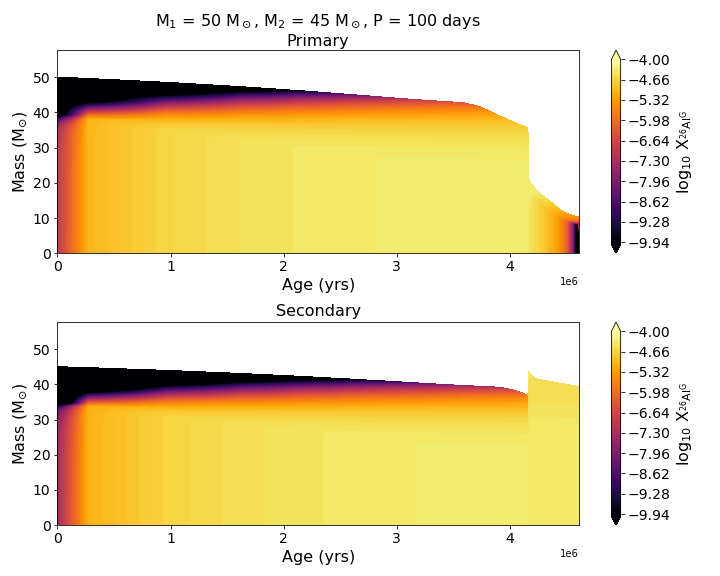
\includegraphics[width=\textwidth]{figures/results1/fig_Al26_Age_M50_P100.png}
        \captionsetup{width=.9\columnwidth}
        \caption{$^{26}$Al composition for the P = 100 days binary simulation.}
        \label{subfig:50Msol_Al26_Bin}
    \end{subfigure}
\caption{As figure \ref{fig:20Msol_Composition} for the M$_1$ = 50 M$_{\sun}$ system.}
\label{fig:50Msol_Composition}
\end{figure*}

The effects of binary interaction on $^{26}$Al yield was found to differ significantly between each primary mass: increasing for the 20 M$_{\sun}$ system, but decreasing for the 50 M$_{\sun}$ system.
The following sections examine each result in turn.

\subsection{20 M$_{\sun}$} \label{20Msol}

\subsubsection{Single Star Evolution}

% Evolution
Figure \ref{subfig:20Msol_HR_Sin} shows the evolution of both the 20 M$_{\sun}$ primary and 18 M$_{\sun}$ secondary as non-interacting single stars.
Initially, both stars move across the main sequence, producing $^{26}$Al in the core (see figure \ref{subfig:20Msol_Al26_Sin}).
The primary star exhausts core hydrogen at $\sim$8.5 Myr (see figure \ref{subfig:20Msol_He4_Sin}) and enters the next stage of its evolution, cooling and expanding at roughly constant luminosity.
Luminosity then increases coinciding with the ignition of helium at $\sim$9.2 Myr.
During this stage, $^{26}$Al is destroyed in the core. Mixing within the stellar envelope also brings some to the surface, where it is ejected by stellar winds (see figure \ref{subfig:20Msol_Al26_Sin}).
The simulation terminates once the primary completes core helium burning at $\sim$10 Myr (see figure \ref{subfig:20Msol_He4_Sin}).

% Yields
The primary loses 4.82 M$_{\sun}$ during single star evolution, ejecting $2.35\times10^{-5}$ M$_{\sun}$ of $^{26}$Al. Note that this is an underestimate because there is still some surface $^{26}$Al remaining at end of the simulation.
However, since the remaining lifetime of the star is at most a few thousand years \citep{Iliadis2015}, there will be minimal additional $^{26}$Al yields before the supernova.

\subsubsection{Binary Star Evolution}

Figure \ref{subfig:20Msol_HR_Bin} shows the evolution of the same stars in a close binary system with an initial period of 100 days.
The stars evolve as above until $\sim$8.5 Myr when the primary exhausts core hydrogen, expands, and fills its Roche lobe (see figure \ref{subfig:20Msol_RLOF}).
Material is exchanged in a single instance of case B mass transfer, which dramatically alters the evolution tracks of both stars.
Figures \ref{subfig:20Msol_He4_Sin} and \ref{subfig:20Msol_He4_Bin} show that the primary's core is largely unaltered while almost the entire envelope is stripped from the star.
The secondary, meanwhile, is rejuvenated by mixing in some of the hydrogen from the accreted material, thus extending its main-sequence lifespan (see \cite{2007MNRAS.376...61D} for more details on this phenomenon).

% Primary yields.
About 12 M$_{\sun}$ of material with a mean $^{26}$Al abundance between $\sim$10$^{-5}$ to $\sim$10$^{-4}$ is lost from the primary, half of which is accreted onto the secondary. The other half is ejected, giving a primary yield of $9.04\times10^{-5}$ M$_{\sun}$ (nearly 4$\times$ the single star yield).
% Secondary yields.
The secondary yields are also increased due to ejection of accreted $^{26}$Al from the surface (see table \ref{tab:data1}).
However, there is little value in comparing these yields at this stage since the secondary evolution was cut short. Continued secondary evolution is discussed in more detail below (see section \ref{Secondaries}).

\subsection{50 M$_{\sun}$}

\subsubsection{Single Star Evolution}

% Evolution
Figure \ref{subfig:50Msol_HR_Sin} shows the evolution of both the 50 M$_{\sun}$ primary and 45 M$_{\sun}$ secondary as non-interacting single stars.
Compared to the $\sim$20 M$_{\sun}$ stars, these stars evolve much faster, lasting only 4.61 Myr before exhausting core helium in the primary.
Note that as a result, both stars complete hydrogen-burning during the same simulation, although the secondary does not complete helium-burning.
Over the course of main sequence evolution, $^{26}$Al is produced in the convective cores which quickly reaches a composition approaching $\sim$10$^{-4}$ in the first Myr.
By $\sim$3.5 Myr for the primary and $\sim$4.0 Myr for the secondary, stellar winds have completely ejected the upper envelope (see figure \ref{subfig:50Msol_Al26_Sin}) and begin ejecting $^{26}$Al. About 10 M$_{\sun}$ is lost from the primary overall during this stage.
Once helium-burning begins in the primary at $\sim$4.2 Myr (see figure \ref{subfig:50Msol_He4_Sin}), stellar winds become much stronger and the star ejects both its entire envelope and the hydrogen shell, leaving the hot, helium-burning core behind as a WR star \citep[see][]{Carroll2007}.
A further $\sim$30 M$_{\sun}$ of material is lost from the primary during this stage.

% Yields
The primary loses 39.68 M$_{\sun}$ during single star evolution, ejecting $9.23\times10^{-4}$ M$_{\sun}$ of $^{26}$Al.
The secondary loses 30.26 M$_{\sun}$ over the same period, ejecting $6.96\times10^{-4}$ M$_{\sun}$ of $^{26}$Al.
The combined $^{26}$Al yield is $1.62\times10^{-3}$ M$_{\sun}$. Since both stars became WR stars, continued evolution is unlikely to yield much more $^{26}$Al before the supernova for either star.

\subsubsection{Binary Star Evolution}

Figure \ref{subfig:50Msol_HR_Bin} shows the evolution of the same stars in a close binary system with an initial period of 100 days.
Mass transfer occurs at $\sim$4.2 Myr when the primary exhausts core hydrogen, expands, and fills its Roche lobe (see figure \ref{subfig:50Msol_RLOF}).
Since stars of this mass become WR, the mass loss profile of the primary is almost identical to its single star evolution (compare figures \ref{subfig:50Msol_He4_Sin} \& \ref{subfig:50Msol_He4_Bin}). Note, however, that some of this lost mass is accreted onto the secondary and does not contribute to yields. Thus, the primary yield is reduced to by about a third to $6.53\times10^{-04}$.

As in the 18 M$_{\sun}$ case, the 45 M$_{\sun}$ secondary's core is rejuvenated by accreted hydrogen \citep[see][]{2007MNRAS.376...61D}. The resulting extension of its main sequence lifespan goes beyond the length of the simulation.
This leads to dramatically reduced secondary yields during the simulated period (see table \ref{tab:data1}), however this is misleading since continued secondary evolution through the WR stage would eject the accreted $^{26}$Al leading to a total yield comparable to the combined single star yield ($\sim$10$^{-3}$ M$_{\sun}$).
However, this would not be the case for systems with a WR primary and a lower mass secondary star that does not become WR even after accreting material.

\subsection{Varying Orbital Period} \label{Period}

\begin{figure}
    \centering
    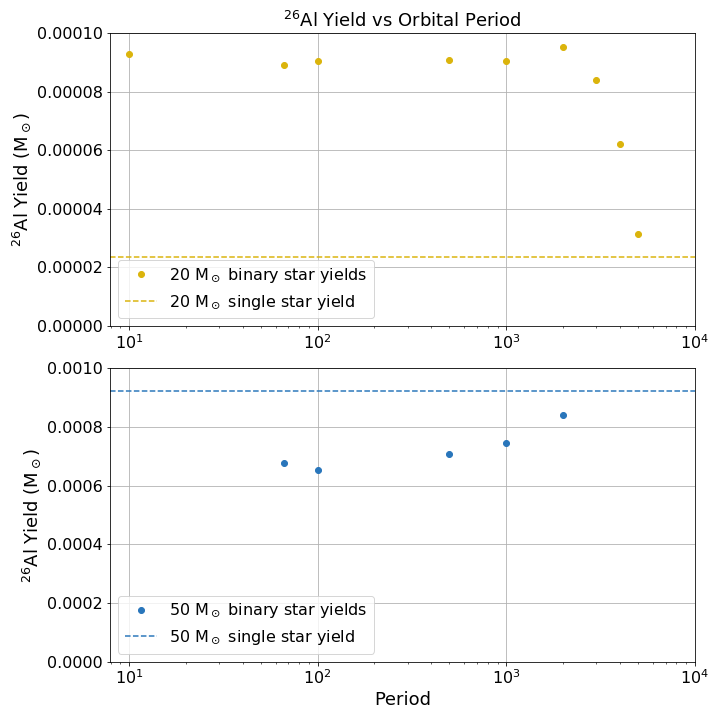
\includegraphics[width=\columnwidth]{figures/results1/fig_YieldvsPeriod.png}
    \captionsetup{width=\columnwidth}
    \caption{$^{26}$Al yield from binary systems of primary masses 20 M$_{\sun}$ and 50 M$_{\sun}$ against orbital period.}
    \label{fig:Period}
\end{figure}

While the basic result of the binary interaction changes depending on the mass of the star in question, the details of the mass transfer depend on the separation between the stars, or equivalently, their orbital period\footnote{Period $P$ and separation $a$ are fundamentally linked by \textit{Kepler's Third Law}: $P^2 = \frac{4\pi}{GM}a^3$.}.
In particular, more distant stars (i.e. those with longer periods) have larger Roche lobes as estimated by the following equation from \cite{1983ApJ...268..368E}:
\begin{equation}
    \frac{R_{RL}}{a}=\frac{0.49q^{2/3}}{0.6q^{2/3}+\ln{1+q^{1/3}}}
\end{equation}
where $R_{RL}$ approximates the Roche lobe radius, $a$ is the separation between stars, and $q$ is the mass ratio $\frac{M_1}{M_2}$.
Thus, they will need to expand to a larger radius to initiate mass transfer than stars with a shorter period.

The effect of the initial period on $^{26}$Al yield was investigated for initial periods 10, 66.2\footnotemark, 100, 500, 1000, and 2000 days.
The key result is that mass transfer occurs sooner in the evolution of each star for systems with a shorter initial period, as can be seen in figure \ref{fig:Period_HR}.
\footnotetext{P = 66.2 days was chosen to allow a direct comparison with a similar simulation by \cite{2019ApJ...884...38B}.}
Further 20 M$_{\sun}$ simulations were run for 3000, 4000, and 5000 day periods to generate more data for cases with particularly late interaction.
The results can be seen in figure \ref{fig:Period}\footnote{Note that the P = 10 days, M$_1$ = 50 M$_{\sun}$ yield was not included. This is because the system evolved into a contact binary, and thus invalidated the assumption of spherical symmetry used by the code.} and table \ref{tab:data1}.
$^{26}$Al yields were found generally constant with respect to period for case B mass transfer at both masses. Case B was also found to be the most commonly occurring type of mass transfer for a flat distribution of initial periods.

The 20 M$_{\sun}$ primary ejected $\sim$9$\times$10$^{-5}$ M$_{\sun}$ of $^{26}$Al after total mass loss of $\sim$14 M$_{\sun}$ for P $\leq$ 1000 days, compared with 2.35$\times$10$^{-5}$ M$_{\sun}$ from a loss of $\sim$5 M$_{\sun}$ for single star evolution.
At higher periods, less mass was lost as the primary evolved out of RLOF before the mass transfer could complete, leading to yields that approach the single star values as period is increased.

The 50 M$_{\sun}$ stars always lost $\sim$40 M$_{\sun}$ regardless of period.
The primary yields were reduced from 9.23$\times$10$^{-4}$ M$_{\sun}$ to $\sim$6$\times$10$^{-4}$ M$_{\sun}$ for P $\leq$ 1000 days due to accretion onto the secondary.
At higher periods, the secondary accreted less mass and experienced less hydrogen rejuvenation. In the P = 2000 days case, the effect was so minor that the secondary began helium-burning within the simulation and the resulting mass loss led to a combined yield of 1.61$\times$10$^{-3}$ M$_{\sun}$, in-line with the combined single star yield (see table \ref{tab:data1}).

\subsection{Varying Mass Transfer Efficiency}

\begin{figure}
    \centering
    \begin{subfigure}{\columnwidth}
        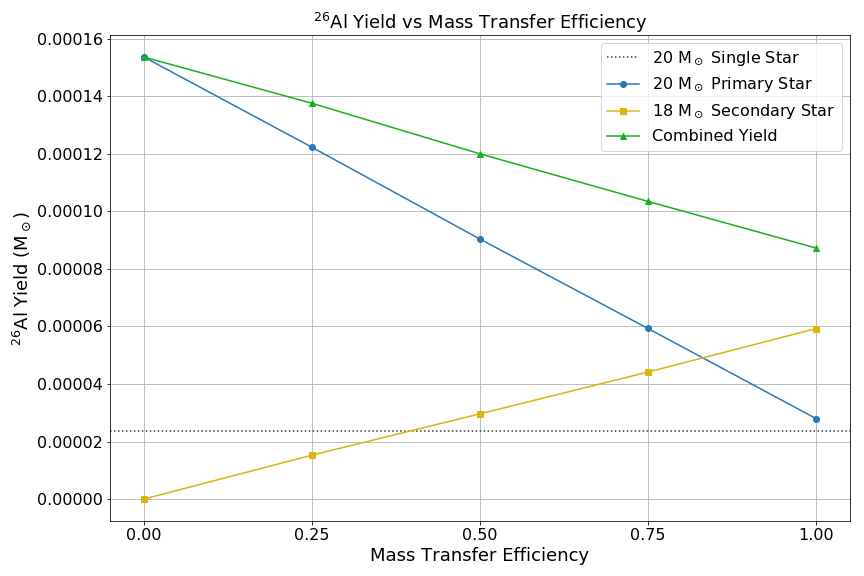
\includegraphics[width=\columnwidth]{figures/results2/fig_YieldvsMTE.png}
        \caption{Primary and secondary $^{26}$Al yields from system evolution up to the end of core helium-burning in the primary star. For comparison, the dotted line shows the yield for the primary evolved as a single star.}
        \label{subfig:MTE1}
    \end{subfigure}
    \begin{subfigure}{\columnwidth}
        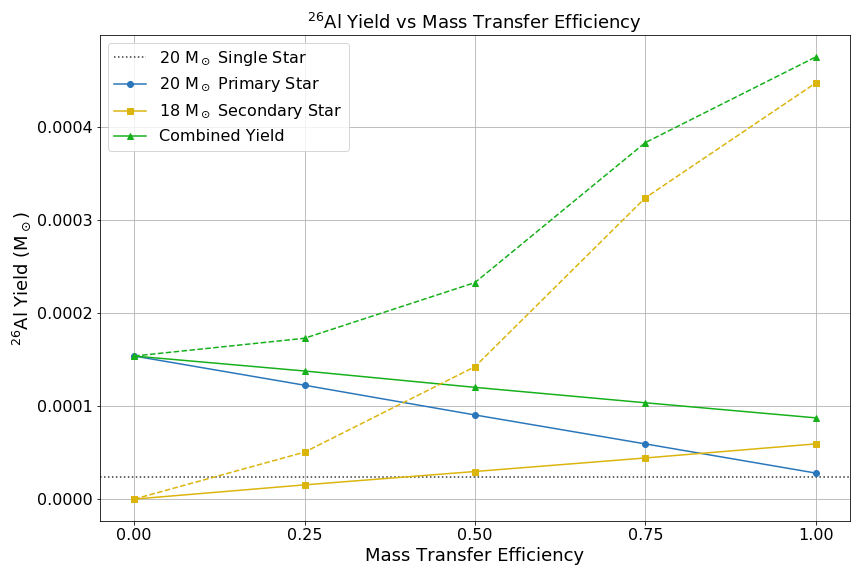
\includegraphics[width=\columnwidth]{figures/results2/fig_YieldvsMTE_2.png}
        \caption{As figure \ref{subfig:MTE1}, with dashed lines showing the binary yields plus additional yields from continued evolution of the secondary star as a single star (i.e. assuming no further binary interaction occurs).}
        \label{subfig:MTE2}
    \end{subfigure}
    \captionsetup{width=\columnwidth}
    \caption{The effect of mass transfer efficiency $\beta$ on $^{26}$Al yield for binary systems with M$_1$ = 20 M$_{\sun}$, M$_2$ = 18 M$_{\sun}$ and an initial period P = 100 days.}
    \label{fig:MTE}
\end{figure}

The effect of mass transfer efficiency $\beta$ on $^{26}$Al yield was investigated using values of $\beta$: 0.00, 0.25, 0.50, 0.75, and 1.00.
Given the minimal effect of binary interactions on the 50 M$_{\sun}$ system (see above), these simulations focused only on the 20 M$_{\sun}$ system at a period of 100 days (this corresponds to case B mass transfer, found above to be the most common -- see section \ref{Period}.).

The results can be seen in figure \ref{subfig:MTE1} and table \ref{tab:data2}.
There are two key points:
\begin{enumerate}
    \item Yields are increased (compared to single star yields) regardless of $\beta$ due to increased surface $^{26}$Al abundance on both stars after RLOF.
    \item The mass lost from the primary is the same in each case ($\sim$12 M$_{\sun}$ from RLOF). Since RLOF yield is proportional to both mass lost and $\beta$ there is a linear decrease in primary yields with increased $\beta$. Conversely, there is a linear increase in secondary yields due to wind mass loss rates increasing with angular momentum as mass is accreted (see section \ref{Method2}).
\end{enumerate}

While the combined yields were found to decrease with $\beta$ (from 1.54$\times$10$^{-4}$ at $\beta$ = 0 to 8.93$\times$10$^{-5}$ at $\beta$ = 1) the increased mass loss rates after accretion indicate the potential for increased yields from the secondaries, if allowed to complete their evolution.

\subsubsection{Continuing the Secondary Evolution} \label{Secondaries}
Once the primary stars complete core helium burning, the remaining $^{26}$Al yields are limited (see section \ref{20Msol}).
However, the less-evolved secondary stars still retain a significant $^{26}$Al composition at this time, especially in cases with high $\beta$.
To investigate these potential $^{26}$Al yields, the secondary star evolution was completed in single star mode.

The results can be seen in figure \ref{subfig:MTE2} and table \ref{tab:data2}, and indicate that the secondary stars could dramatically increase the system $^{26}$Al yield, if left to evolve without further binary interaction.
%After mass transfer, the secondaries' evolution paths were found to be roughly similar to those of single stars of masses equal to the new masses (see figures \ref{fig:MTE_HR}).
For 0 < $\beta$ $\leq$ 0.50, this led to evolution tracks a little higher in luminosity and evolution speed than the $\beta$ = 0 track, with stronger winds, greater mass loss, and correspondingly higher yields.
For $\beta$ $\geq$ 0.75, the secondary stars reached sufficient masses to become WR stars: ejecting nearly all of the $^{26}$Al produced by both stars.
At $\beta$ = 1, the secondary star ejected 18.2 M$_{\sun}$ of material during the continued evolution (more than its initial mass), resulting in a combined system $^{26}$Al yield of 4.75$\times$10$^{-4}$ (> 3 times the $\beta=0$ yield).      % ~1580/1500 (+ 80)
\section{Discussion} % Approx word count = 500 words  (total = 3250)

Comparing the results of this study with those of \cite{2019ApJ...884...38B}, there is qualitative agreement on the effects of case B mass transfer on $^{26}$Al wind yields:
\begin{enumerate}
    \item Both studies found that yields increased for the 20 M$_{\sun}$ primary but decreased for the 50 M$_{\sun}$ primary.
    \item Yields were found to increase significantly for 20 M$_{\sun}$ systems, while the 50 \& 45 M$_{\sun}$ WR stars were found to have the same yields regardless of whether the stars transferred mass. This supports the initial mass function described by \cite{2019ApJ...884...38B}, which indicates that the effect of mass transfer on wind yields becomes negligible for systems with initial masses above $\sim$35 M$_{\sun}$ and mass ratio $0.5 < q < 0.9$.
\end{enumerate}

It is worth noting that this study generally finds much higher yields (by 1 or 2 orders of magnitude) for all simulations\footnote{Most simulations in \cite{2019ApJ...884...38B} use $\beta$ = 1, which would decrease primary yields. However, since the yield difference is also found in single star models, binary parameters cannot be the cause.} despite both studies evolving models up to the end of core helium-burning.
\cite{2019ApJ...884...38B} discusses the potential effects of uncertainties in the main $^{26}$Al production channel: $^{25}$Mg$(p,\gamma)^{26}$Al, finding a 2 orders of magnitude shift in core $^{26}$Al abundance as the reaction rate is varied.
It is thus likely that differences in the reaction rates used are the cause of the yield difference (or at least a major factor), but this has not been confirmed.

\cite{2019ApJ...884...38B} also briefly\footnotemark investigates the effects of varying mass transfer efficiency $\beta$ on $^{26}$Al yield for a binary system with M$_1$ = 20 M$_{\sun}$, M$_2$ = 18 M$_{\sun}$, and P = 18.4 days. They found that primary yields increased linearly between $1.41\times10^{-6}$ and $2.00\times10^{-6}$ M$_{\sun}$ with decreasing $\beta$.
\footnotetext{The scheme used treated the mass transfer as an instantaneous event. This assumption gives a good yield estimate, but ignores some of the complexities such as continued $^{26}$Al decay during RLOF.}
A linear trend, though steeper, was also observed in this study: between $1.54\times10^{-4}$ and $2.80\times10^{-5}$ M$_{\sun}$.
However, the more significant result was actually in the secondary stars, which showed a non-linear relationship with $\beta$ (see figure \ref{subfig:MTE2}) due to the increase in wind mass loss rates and surface $^{26}$Al composition in the mass-gaining stars.
This meant that decreased primary yields actually corresponded to higher overall yields once both stars completed their evolution.
Given the number of binary parameters to vary, more work is needed to explore how mass transfer efficiency affects the yields of other systems.

\subsection{The Fate of Secondary Stars after RLOF}

The binary simulations terminated at the end of core helium-burning in the primary, at which point its remaining lifetime is relatively short. Massive stars end their lives in a supernova, leaving behind either a neutron star or (for initial masses greater than $\sim$25 M$_{\sun}$) a black hole \citep[see][]{Carroll2007,Iliadis2015}.
If the secondary does not merge with the primary before the supernova, there are three possible fates:
\begin{enumerate}
    \item The supernova destroys the secondary.
    \item The secondary survives the supernova, remaining in an interacting binary system with the primary remnant.
    \item The secondary survives the supernova, but is pushed far enough away that it completes its evolution without further binary interaction.
\end{enumerate}

Due to time limitations, and the inability to simulate contact binaries\footnotemark, this study focused on the third possibility.
\cite{2015A&A...584A..11L} provides evidence that secondary stars can complete their evolution undisturbed even after their partner star reaches supernova. However, it was not determined that this evolution path was the correct one for the systems in question.
Nonetheless, the high yields from continued secondary evolution point to a potential source of $^{26}$Al from massive binaries not immediately evident from just the primary star behaviour.
\footnotetext{While contact binaries invalidate the spherical symmetry assumption used by STARS, mass-transfer from the secondary back to the primary \emph{could} be simulated in STARS and produce valid results as long as both STARS do not simultaneously fill their Roche lobes. This presents a promising subject for future work.}

\subsection{Rotating vs non-rotating binaries}

This study used non-rotating models for simplicity, but nearly all actual stars will experience some degree of rotation.
The effects of rotation on stellar evolution for both single and binary stars is explored in \cite{2019EAS....82..137M}.
One key difference relevant to $^{26}$Al is that rotating stars experience larger regions of homogenised composition due to rotational mixing.
Depending on whether this mixing dilutes or enriches the $^{26}$Al content in the ejected material, it could lead to either increased or decreased yields. For binary stars, the effect will also depend on the timing of RLOF.

In the case of the single 20 M$_{\sun}$ star (see figure \ref{subfig:50Msol_Al26_Sin}), a larger mixed region would enrich the material ejected by winds and produce a higher yield. In the binary counterpart (see figure \ref{subfig:50Msol_Al26_Bin}), it seems unlikely that a larger mixed region would affect yields since RLOF ejects the entire convective region and the layers below.
Similarly, while WR stars are known to have very strong rotation \citep{Carroll2007}, the complete ejection of their envelope would likely render the effects of increased mixing irrelevant to the $^{26}$Al yields in both single and binary models.
The results of this study should be taken as qualitatively representative of the effects of binary interactions, but future work is needed to fully quantify the effect of binary interactions on $^{26}$Al yields.   % ~ 740/ 750 (- 10)
\section{Conclusion} % Approx word count = 250 words (total = 3500)

% Basic Result
The effects of mass transfer via RLOF on $^{26}$Al wind yields from non-rotating massive binary stars was investigated.
The initial orbital period was found to determine when RLOF occurred in the star's evolution (i.e. whether mass transfer was case B, C, etc.) but had minimal effect on yields beyond that.
For case B mass transfer, yields were found to increase by a factor of $\sim$4 for a mass-losing 20 M$_{\sun}$ star at mass transfer efficiency $\beta$ = 0.5.
For case C mass transfer, the yields were comparable to those of their single star counterparts due to a combination of reduced mass loss and increased $^{26}$Al decay.
If the star would normally evolve into a Wolf-Rayet star (initial mass > $\sim$20 M$_{\sun}$), $^{26}$Al yields were instead decreased due to accretion of material that would otherwise be ejected.
Yields were also found to increase for the mass-gaining star due to increased surface $^{26}$Al abundance and increased mass loss rates resulting from the transfer of angular momentum.
Mass-gaining stars that would normally evolve into WR stars were found to have their main sequence lifespan extended, but as above their yields remained largely unaffected.

By increasing $\beta$, it was found that the reduced yields from mass-losing stars due to increased accretion onto a companion was ultimately outweighed by the increase in the companion's yields (under the assumption that the companion completes its evolution without continued binary interaction).
The total yield for a 20 \& 18 M$_{\sun}$ system was found to increase by a factor $\sim$3 from 1.54$\times$10$^{-4}$ ($\beta$ = 0) to 4.75$\times$10$^{-4}$ M$_{\sun}$ ($\beta$ = 1).
This increase was found to be non-linear, and was especially significant for companion stars that gained sufficient mass to become WR stars.   % ~ 280/ 250 (+ 30)
%                             %TOT ~3830/3500 (+330)

%%%%%%%%%%%%%%%%%%%%%%%%%%%%%%%%%%%%%%%%%%%%%%%%%%

%%%%%%%%%%%%%%%%%%%% REFERENCES %%%%%%%%%%%%%%%%%%

% The best way to enter references is to use BibTeX:

\bibliographystyle{mnras}
\bibliography{bibliography}


% Alternatively you could enter them by hand, like this:
% This method is tedious and prone to error if you have lots of references
%\begin{thebibliography}{99}
%\bibitem[\protect\citeauthoryear{Author}{2012}]{Author2012}
%Author A.~N., 2013, Journal of Improbable Astronomy, 1, 1
%\bibitem[\protect\citeauthoryear{Others}{2013}]{Others2013}
%Others S., 2012, Journal of Interesting Stuff, 17, 198
%\end{thebibliography}

%%%%%%%%%%%%%%%%%%%%%%%%%%%%%%%%%%%%%%%%%%%%%%%%%%

%%%%%%%%%%%%%%%%% APPENDICES %%%%%%%%%%%%%%%%%%%%%

\appendix
\section{Additional Figures}

\begin{figure*}
    \centering
    \begin{subfigure}{\columnwidth}
        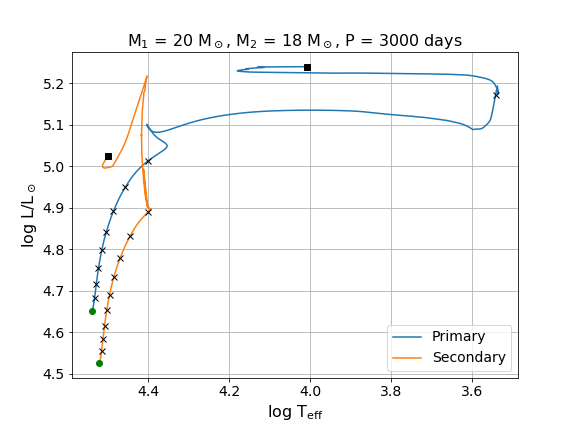
\includegraphics[width=\columnwidth]{figures/results1/fig_HR_M20_P3000.png}
        \label{subfig:20Msol_P3000_HR}
    \end{subfigure}
    \begin{subfigure}{\columnwidth}
        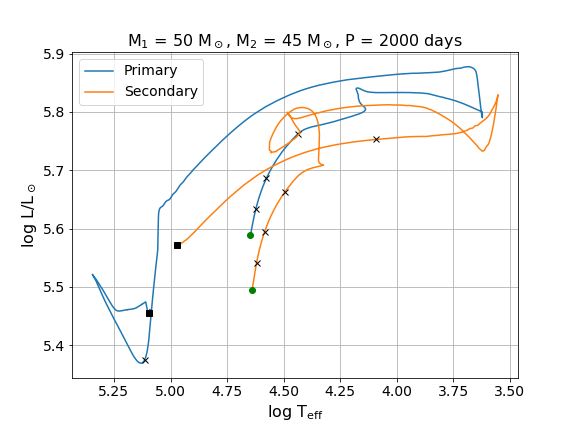
\includegraphics[width=\columnwidth]{figures/results1/fig_HR_M50_P2000.png}
        \label{subfig:50Msol_P2000_HR}
    \end{subfigure}
    
    \begin{subfigure}{\columnwidth}
        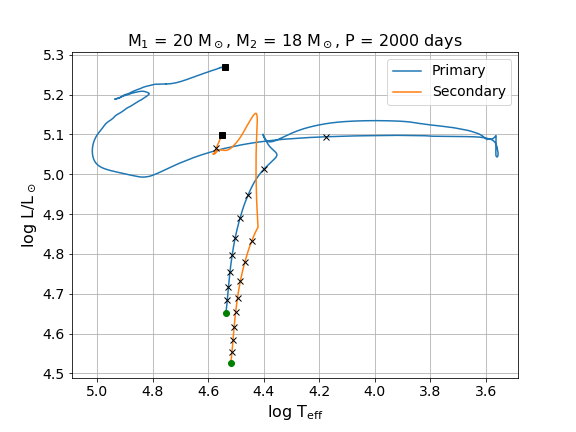
\includegraphics[width=\columnwidth]{figures/results1/fig_HR_M20_P2000.png}
        \label{subfig:20Msol_P2000_HR}
    \end{subfigure}
    \begin{subfigure}{\columnwidth}
        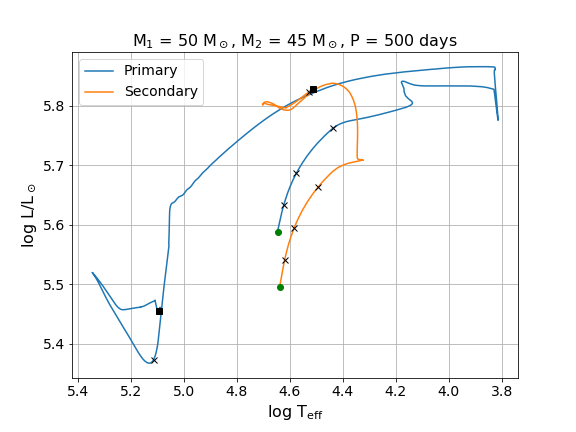
\includegraphics[width=\columnwidth]{figures/results1/fig_HR_M50_P500.png}
        \label{subfig:50Msol_P500_HR}
    \end{subfigure}
    
    \begin{subfigure}{\columnwidth}
        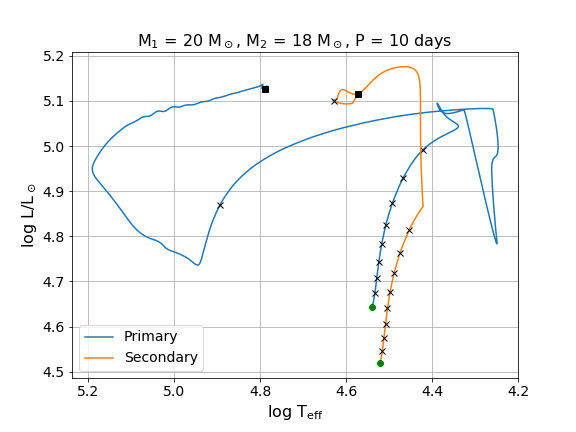
\includegraphics[width=\columnwidth]{figures/results1/fig_HR_M20_P10.png}
        \label{subfig:20Msol_P10_HR}
    \end{subfigure}
    \begin{subfigure}{\columnwidth}
        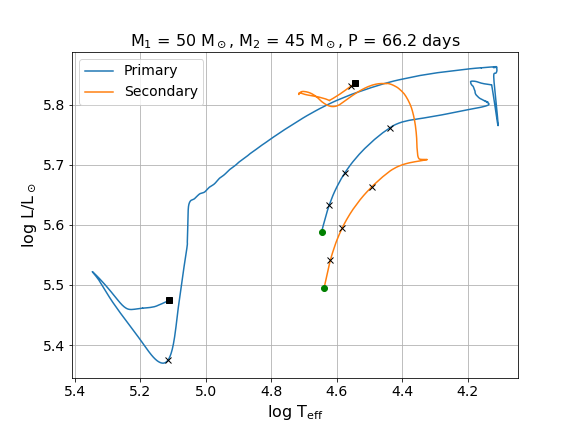
\includegraphics[width=\columnwidth]{figures/results1/fig_HR_M50_P66.png}
        \label{subfig:50Msol_P66_HR}
    \end{subfigure}
    
\caption{HR diagrams comparing the evolution of M$_1$ = 20 M$_\sun$ (left) and M$_1$ = 50 M$_\sun$ (right) binary systems at different initial periods. The shorter the period, the sooner in their evolution RLOF occurs. Note that as massive stars have higher luminosities, the secondary tracks move upwards as mass is accreted. The HR diagrams are as figure \ref{fig:SinglevsBinary}. For the M$_1$ = 20 M$_\sun$ system, mass transfer was case C (RLOF during helium-burning) for P > 2000 days, and case B for 10 < P < 2000 days. P = 2000 days provided an edge case where RLOF coincided with the ignition of helium. For the M$_1$ = 50 M$_\sun$ system, mass transfer was case B for P > 10 days, and case A for P = 10 days (not pictured). In this latter simulation, both stars filled their Roche lobes simultaneously, forming a contact binary and rendering the HR diagram invalid beyond that point. Note that for P = 2000, the secondary's accretion is limited enough that it begins its WR evolution even after rejuvenation of core hydrogen extends its main sequence lifespan.}
\label{fig:Period_HR}
\end{figure*}

\begin{figure*}
    \centering
    \begin{subfigure}{\columnwidth}
        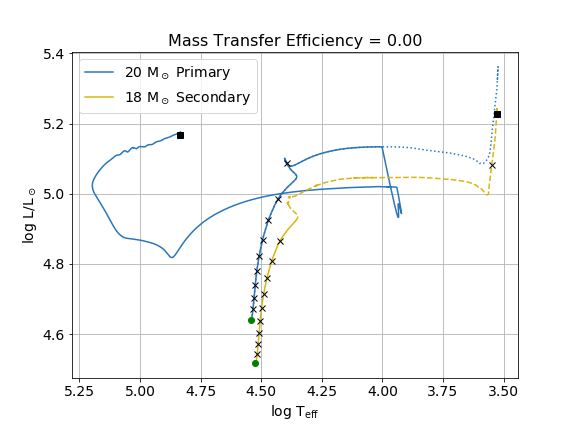
\includegraphics[width=\columnwidth]{figures/results2/fig_HR_MassTransfer_0.png}
        \label{subfig:MTE0_HR}
    \end{subfigure}
    \begin{subfigure}{\columnwidth}
        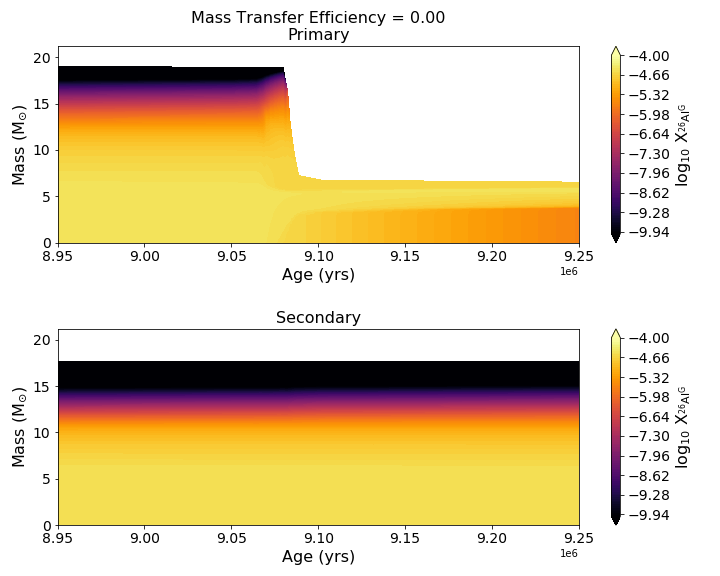
\includegraphics[width=\columnwidth]{figures/results2/fig_Al26_MassTransfer_0.png}
        \label{subfig:MTE0_Al26}
    \end{subfigure}
    
    \begin{subfigure}{\columnwidth}
        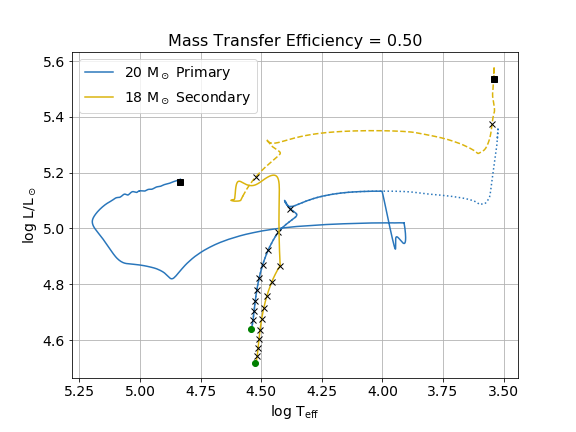
\includegraphics[width=\columnwidth]{figures/results2/fig_HR_MassTransfer_50.png}
        \label{subfig:MTE50_HR}
    \end{subfigure}
    \begin{subfigure}{\columnwidth}
        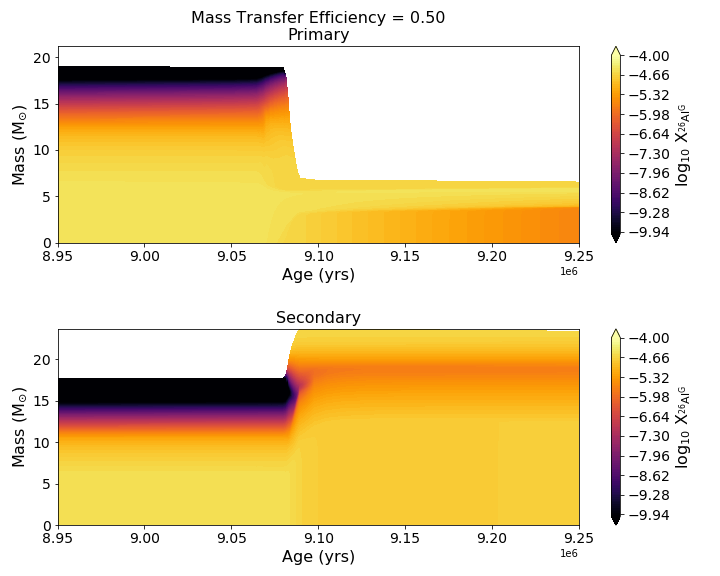
\includegraphics[width=\columnwidth]{figures/results2/fig_Al26_MassTransfer_50.png}
        \label{subfig:MTE50_Al26}
    \end{subfigure}
    
    \begin{subfigure}{\columnwidth}
        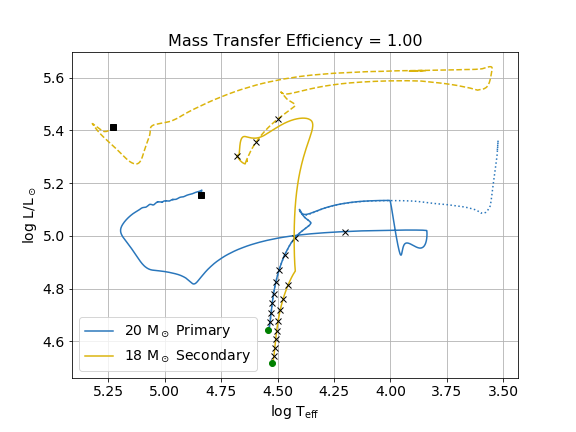
\includegraphics[width=\columnwidth]{figures/results2/fig_HR_MassTransfer_100.png}
        \label{subfig:MTE100_HR}
    \end{subfigure}
    \begin{subfigure}{\columnwidth}
        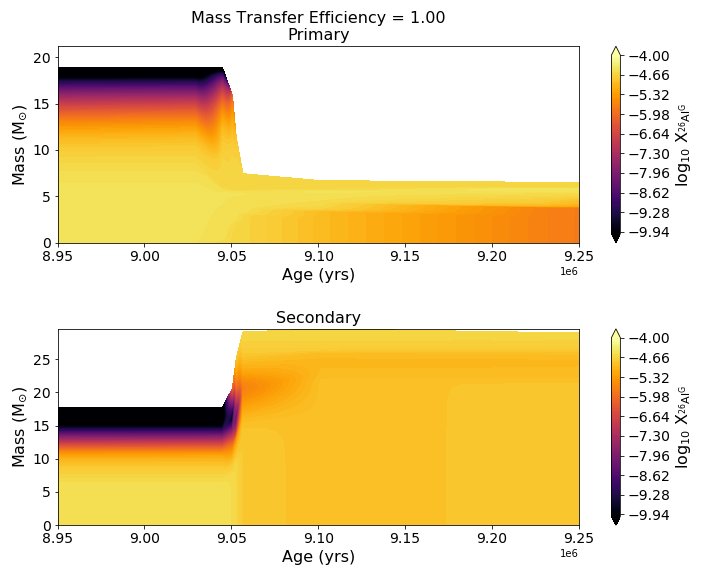
\includegraphics[width=\columnwidth]{figures/results2/fig_Al26_MassTransfer_100.png}
        \label{subfig:MTE100_Al26}
    \end{subfigure}
\caption{HR diagrams (left) and $^{26}$Al composition diagrams (right) comparing the evolution of binary stars undergoing non-conservative mass transfer (top), partially conservative mass transfer (middle), and fully conservative mass transfer (bottom).
For the HR diagrams: the dotted blue line depicts the evolution track of a single star counterpart to the primary, and the dashed yellow line shows the continued single-star evolution of the secondary star after mass transfer.
The composition diagrams are as figures \ref{fig:20Msol_Composition} \& \ref{fig:50Msol_Composition}, but focused only on the RLOF stage of evolution.
Each simulation has initial primary mass 20 M$_{\sun}$, mass ratio q = 0.9, and initial orbital period P = 100 days.}
\label{fig:MTE_HR}
\end{figure*}
\section{Tables of Results}

\begin{table*}
 \caption{Tabulated data for simulations varying the initial period of the orbit P$_{init}$ for two initial primary star masses M$_{init}$.
 All simulations used mass ratio q = 0.9, and mass transfer efficiency $\beta$ = 0.5.
 $\Delta$M$_1$ \& $\Delta$M$_2$ give the change in mass for the primary and secondary stars respectively, while $\Delta$t gives the time difference between the start and end of the simulation.
  $^{26}$Al$_1$, $^{26}$Al$_2$, and $^{26}$Al$_{tot}$ give the primary, secondary, and combined $^{26}$Al yields respectively.
 }
 \label{tab:data1}
 \begin{tabular}{lccccccc}
  \hline
  M$_{init}$ & P$_{init}$ & $\Delta$M$_1$ & $\Delta$M$_2$ & $\Delta$t & $^{26}$Al$_1$ & $^{26}$Al$_2$ & $^{26}$Al$_{tot}$ \\
  M$_{\sun}$ & days & M$_{\sun}$ & M$_{\sun}$  & Myr & M$_{\sun}$ & M$_{\sun}$ & M$_{\sun}$ \\
  \hline
  20 & 10$^{77}$ & -4.82 & -0.67 & 10.03 & 2.35e-05 & 6.54e-12 & 2.35e-05 \\
   & 5000 & -5.82 & -0.67 & 10.00 & 3.15e-05 & 6.57e-12 & 3.15e-05 \\
   & 4000 & -10.71 & +1.57 & 10.00 & 6.20e-05 & 3.45e-08 & 6.21e-05 \\
   & 3000 & -11.98 & +2.24 & 9.99 & 8.40e-05 & 7.79e-07 & 8.48e-05 \\
   & 2000 & -13.36 & +4.17 & 9.97 & 9.53e-05 & 9.07e-06 & 1.04e-04 \\
   & 1000 & -14.13 & +4.35 & 10.00 & 9.05e-05 & 2.67e-05 & 1.17e-04 \\
   & 500 & -14.29 & +4.42 & 9.97 & 9.08e-05 & 2.80e-05 & 1.19e-04 \\
   & 100 & -14.31 & +4.41 & 10.00 & 9.04e-05 & 2.96e-05 & 1.20e-04 \\
   & 66.2 & -14.38 & +4.43 & 10.00 & 8.90e-05 & 2.93e-05 & 1.18e-04 \\
   & 10 & -14.78 & +4.47 & 9.99 & 9.27e-05 & 3.18e-05 & 1.24e-04 \\
  \hline
  50 & 10$^{77}$ & -39.68 & -30.26 & 4.61 & 9.23e-04 & 6.96e-04 & 1.62e-03 \\
   & 2000 & -39.83 & -28.46 & 4.61 & 8.42e-04 & 7.68e-04 & 1.61e-03 \\
   & 1000 & -39.84 & -6.03 & 4.61 & 7.46e-04 & 1.15e-04 & 8.61e-04 \\
   & 500 & -39.85 & -5.82 & 4.61 & 7.07e-04 & 1.67e-04 & 8.73e-04 \\
   & 100 & -39.74 & -5.66 & 4.61 & 6.53e-04 & 1.74e-04 & 8.27e-04 \\
   & 66.2 & -39.82 & -6.04 & 4.61 & 6.79e-04 & 1.94e-04 & 8.73e-04 \\
%   & 10 & -29.01 & -13.36 & 4.21 & 5.85e-04 & 1.57e-04 & 7.42e-04 \\ %% NOTE: Data invalid due to contact binary.
  \hline
 \end{tabular}
\end{table*}

\begin{table*}
 \caption{Tabulated data for simulations varying the mass transfer efficiency $\beta$.
 All simulations are for an initial primary star mass M$_1$ = 20 M$_{\sun}$ with mass ratio q = 0.9 and initial period P = 100 days.
 Binary simulations were run up to the end of core helium burning in the primary star.
 Continued single-star simulations for the secondaries were run up to the same stage: data from these simulations is marked (cont.).
 $\Delta$M$_1$ \& $\Delta$M$_2$ give the change in mass for the primary and secondary stars respectively, while $\Delta$t gives the time difference between the start and end of the simulation.
 $^{26}$Al$_1$, $^{26}$Al$_2$, and $^{26}$Al$_{tot}$ give the primary, secondary, and combined $^{26}$Al yields respectively.
 }
 \label{tab:data2}
 \begin{tabular}{lccccccccc}
  \hline
  $\beta$ & $\Delta$M$_1$ & $\Delta$M$_2$ & $\Delta$M$_2$ (cont.) & $\Delta$t & $\Delta$t (cont.) & $^{26}$Al$_1$ & $^{26}$Al$_2$ & $^{26}$Al$_{tot}$ & $^{26}$Al$_{tot}$ (cont.) \\
  & M$_{\sun}$ & M$_{\sun}$ & M$_{\sun}$  & Myr & Myr & M$_{\sun}$ & M$_{\sun}$ & M$_{\sun}$ & M$_{\sun}$ \\
  \hline
  0.00 & -14.31 & -0.66 &  -2.59 & 10.00 & 1.28 & 1.54e-04 & 7.22e-12 & 1.54e-04 & 1.54e-04 \\
  0.25 & -14.34 & +2.04 &  -4.81 & 9.97 & 2.11 & 1.22e-04 & 1.53e-05 & 1.38e-04 & 1.73e-04 \\
  0.50 & -14.31 & +4.41 &  -9.75 & 10.00 & 2.64 & 9.04e-05 & 2.96e-05 & 1.20e-04 & 2.33e-04 \\
  0.75 & -14.32 & +6.80 & -15.59 & 9.97 & 2.94 & 5.93e-05 & 4.42e-05 & 1.03e-04 & 3.83e-04 \\
  1.00 & -14.33 & +9.16 & -18.19 & 9.97 & 3.00 & 2.80e-05 & 5.93e-05 & 8.73e-05 & 4.75e-04 \\
  \hline
 \end{tabular}
\end{table*}

%%%%%%%%%%%%%%%%%%%%%%%%%%%%%%%%%%%%%%%%%%%%%%%%%%


% Don't change these lines
\bsp	% typesetting comment
\label{lastpage}
\end{document}

% End of mnras_template.tex